
\section{Medici\'on corriente de bias y tensi\'on de offset}

\subsection{Introducción}
Las corrientes de \textbf{bias} son las corrientes de polarización de la electrónica dentro de los amplificadores operacionales, en el informe se analizará 2 operacionales, uno con corrientes de bias atribuídas a la corriente de base de un par diferencial de transistores de juntura bipolar a la entrada del mismo y otro implementado con J-FET que si bien teóricamente no debería tener corriente de gate realmente la tiene.
La tension de offset es la diferencia de potencial que se encuentra a la salida del operacional teniendo una tension nula a la entrada.
Otra corriente de interés es la Corriente de offset.
Con el modelo del Op Amp que tiene en cuenta estos fenómenos se puede definir.\newline
 	
 $I_{offSet} \ = \ |I_b^{-}-I_b^{+}|$\ y \ $I_{Bias}= \frac{I_b^-+I_b^{+}}{2}$
\begin{figure}[H]	
	\centering
	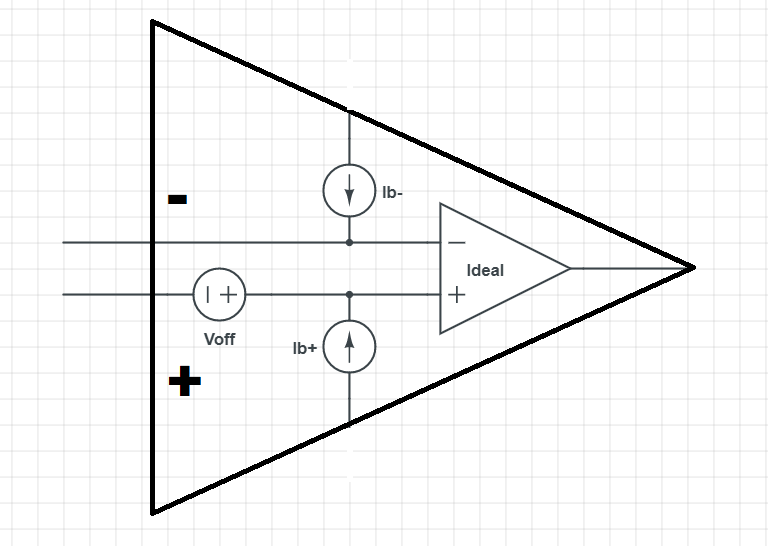
\includegraphics[width=0.7\textwidth]{Ej3/imagenes/opampReal.PNG}
	\caption{Modelo OpAmp con corriente de bias y tensión de offset.}
	\label{fig:OpampBias}
\end{figure}



Se proporcionó el siguiente circuito para medir las corrientes de bias y la tension de offset.

\begin{figure}[H]	
	\centering
	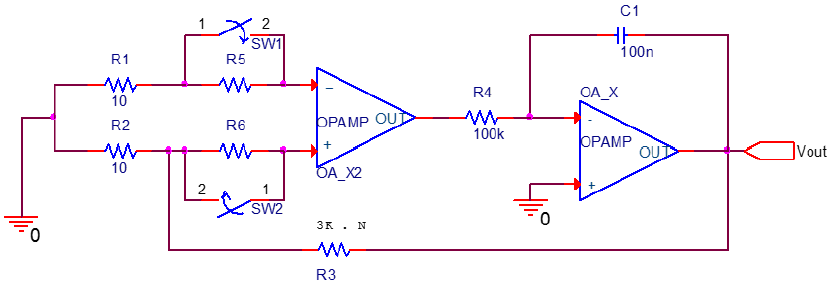
\includegraphics[width=0.7\textwidth]{Ej3/imagenes/CircMedicion.PNG}
	\caption{Circuito de medición.}
	\label{fig:CircMedicion}
\end{figure}

\subsection{Estabilidad}
Se analizó cada módulo del circuito por separado realizando el diagrama de flujo de señal para el análisis de estabilidad.\\
Se comenzó por la segunda parte dado que es necesario un resultado de esta parte para realizar la primera

\begin{figure}[htb]	
	\centering
	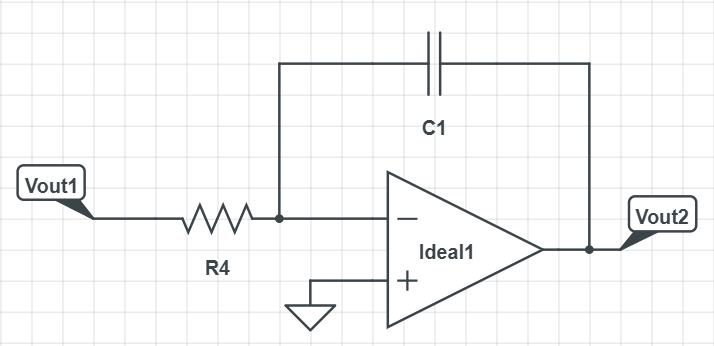
\includegraphics[width=0.7\textwidth]{Ej3/imagenes/SegundaEtapa.PNG}
	\caption{Segunda Etapa.}
	\label{fig:SegundaEtapa}
\end{figure}
La corriente circulara a través de la resistencia y el capacitor.\\
\begin{center}
$ \frac{V_{out_1}-V^-}{R_4} = (V^--V_{out_2})\cdot sc$ \\
\end{center}
 Despejando para \ $V^-$ \ se llega a: \\
\begin{center}
$V^- = V_{out_1} \cdot \frac{1}{scR_4+1}+V_{out_2} \cdot \frac{scR_4}{scR_4+1}$\\\end{center}
y utilizando la ecuación del OpAmp:\\
\begin{center}
$V_{out_2}=A_0 \cdot (-V^-)$
\end{center}
Se llega al siguiente diagrama
\begin{figure}[H]	
	\centering
	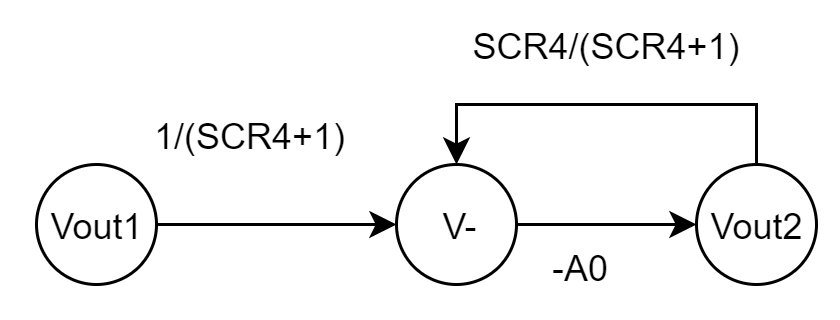
\includegraphics[width=0.7\textwidth]{Ej3/imagenes/SegundaEtapaDiagrama.PNG}
	\caption{Diagrama de flujo de señal de la segunda etapa.}
	\label{fig:SegundaEtapaDiagrama}
\end{figure}
De aqui se puede apreciar que el circuito es estable dado a que la realimentación es negativa y por lo tanto estable, si se invirtiese la entrada, el circuito pasaría a ser inestable\\
Luego analizando la primer etapa
\begin{figure}[H]	
	\centering
	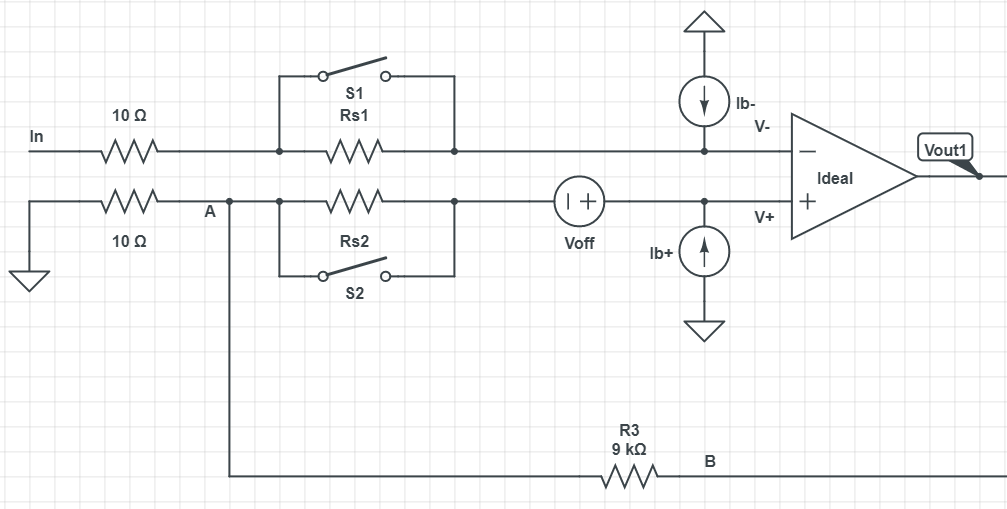
\includegraphics[width=0.7\textwidth]{Ej3/imagenes/PrimeraEtapa.PNG}
	\caption{Primer Etapa.}
	\label{fig:PrimerEtapa}
\end{figure}
Sabiendo que la tensión en B sera el resultado de la configuración inversora de la segunda etapa.\\
\begin{center}$V_{out_1}=A_0 \cdot (V^+ - V^-)$\\\end{center}
\begin{center}$V^+= V_{out_1}\cdot \frac{-1}{SCR_4} \cdot \frac{10}{10+R_3} $\\\end{center}
\begin{center}$V^- = V_+{in}$\\\end{center}
Se obtiene el diagrama de flujo de señal:
\begin{figure}[H]	
	\centering
	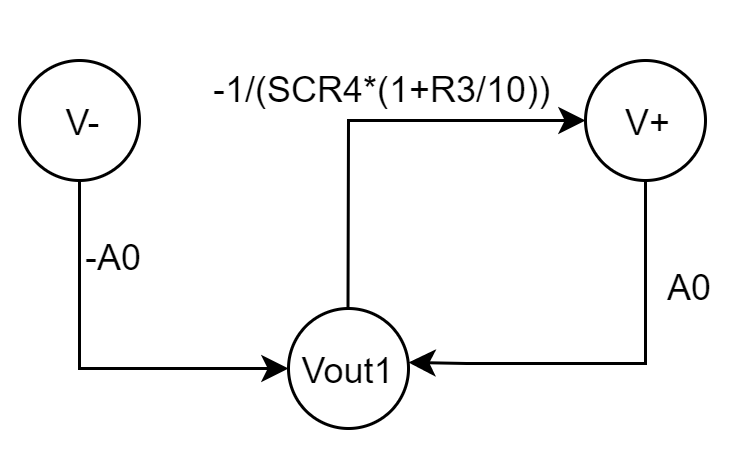
\includegraphics[width=0.7\textwidth]{Ej3/imagenes/PrimerEtapaDiagrama.PNG}
	\caption{Diagrama de flujo de señal de la primer etapa.}
	\label{fig:PrimerEtapaDiagrama}
\end{figure}
El cual también se puede notar que es estable dado a la realimentación negativa, en caso de permutar las entradas cambiarían los signos de los lazos y seria inestable.
Finalmente si se invierten las entradas de ambas etapas en simultaneo también sera inestable dado que si un sub-sistema dentro de un sistema es inestable, el sistema entero lo será.\\
A modo de conclusión se llega a que el la única configuración estable es la original, dado que la permutación de las entradas lleva a situaciones inestables por la realimentación positiva.
\subsection{Deducción de expresiones para medir.}

Teniendo en cuenta el circuito entero de medición, las corrientes de bias y la tension de offset se lo puede modelar de la siguiente manera
\begin{figure}[H]	
	\centering
	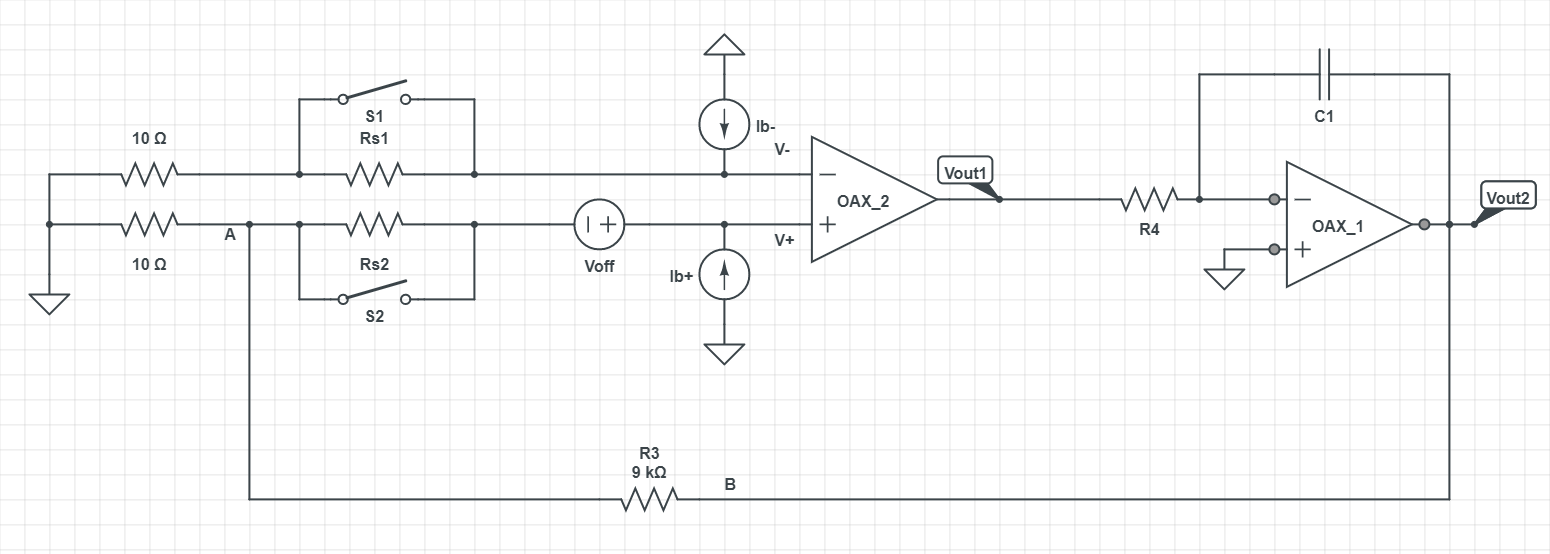
\includegraphics[width=\textwidth]{Ej3/imagenes/Medicion.PNG}
	\caption{Circuito de medición.}
	\label{fig:Medicion}
\end{figure}
El Opamp a medir será el OAX-2
\begin{center}$V_{out_1}=A_0 \cdot (V^+ - V^-)$\\\end{center}
Dado a que la corriente de bias es únicamente continua para la segunda etapa el opamp es como si estuviese a lazo abierto\\
\begin{center}$V_{out_2}=A_0 \cdot V_{out_1}$\\\end{center}
\begin{center}$V^-=I_b^- \cdot (R_{s2}+10)$\\\end{center}
\begin{center}$V^+=I_b^+ \cdot R_{s1} +V_A+V_{off}$\\\end{center}
\begin{center}$V_A=V_{out_2} \cdot \frac{1}{1+\frac{10}{R_3}}$\\\end{center}
Despejando para $V_{out_2}$ se llega a:
\begin{center}$V_{out_2}=A_0^2  \cdot \frac{I_b^+ \ R_{s1} -I_b^-\cdot (R_{s2}+10)+V_{off}}{1-A_0^2 \cdot \frac{1}{1+\frac{10}{R_3}}}$\\\end{center}
$\lim_{A_0\to\infty} A_0^2  \cdot \frac{I_b^+ \ R_{s1} -I_b^-\cdot (R_{s2}+10)+V_{off}}{1-A_0^2 \cdot \frac{1}{1+\frac{10}{R_3}}}=-(I_b^+ \ R_{s1} -I_b^-\cdot (R_{s2}+10)+V_{off})\cdot \frac{1}{1+\frac{10}{R_3}} $
Luego cambiando de posición la llave se va a poder medir los diferentes observables de interés del circuito.\\
La $V_{off}$ se medirá poniendo en corto $R_{s1}$ y $R_{s2}$ y se despreciará la caída sobre el resistor de 10$\omega$ dado a su pequeño valor y que la corriente de bias también es muy pequeña.\\
\begin{center}$V_{off}=V_{out_2} \cdot \frac{10}{10+R_3} $\end{center}
Ahora que se tiene un valor de $V_{off}$ se  puede poner en corto S1 ó S2 arbitrariamente y se conseguirá una expresión para $ I_b^+ \ o \  I_b^-$ en función de $V_{off} \ y \ V_{out_2}$
Se tuvo en cuenta elegir un valor de resistencia alto para $R_{s1}$ y $R_{s2}$ talque sea mas apreciable la caída de potencial sobre ellas; se eligió 1 Mega.\\
\begin{center}$I_b^+=\frac{V_{out_2} \cdot \frac{10}{10+R_3}-V_{off}}{R_{s1}}$\end{center}
Para esta expresión se desprecio el valor de $I_b^-$
\begin{center}$I_b^-=\frac{V_{out_2} \cdot \frac{10}{10+R_3}-V_{off}}{R_{s2}+10}$\end{center}

\subsection{Ruido Ambiente.}
La segunda etapa si bien está a laso abierto para las corrientes de bias dado que es de continua se comporta como un filtro para el ruido ambiente que se encuentra a 50Hz,con los valores actuales de resistencia y capacitor atenuará $\approx$ 0.45dB, aumentando el valor del capacitor a 1$\mu F$ será de  $\approx$ 20dB.
Un problema que se presentaría aplicando un capacitor demasiado chico es que el ruido haría mucho mas difícil las mediciones.
El ruido que es introducido por el terminal no inversor del Opamp utilizando superposición se encuentra en una configuración no inversora, que dependiendo de la intensidad del ruido puede invertir el lazo y hacer que el circuito oscile.
\subsection{Resultados.}
\subsubsection{Mediciones}
Se midió el circuito utilizando osciloscopio y se  obtuvo la siguiente tabla.
\begin{table}[H]
\begin{center}
\label{tab:vout}
\caption{Mediciones}
\begin{tabular}{c|c|c|c|}
\hline
\multicolumn{4}{|c|}{\textbf{Mediciones Realizadas}} \\ \hline
 & \multicolumn{3}{c|}{\textbf{Vout}} \\ \cline{2-4} 
Switches & Rs1 y Rs2=0 & RS2 =0 & RS1 =0 \\ \hline
\multicolumn{1}{|c|}{\textbf{Osciloscopio}} & -1.3V & -1.4431V & -1.3903V \\ \hline
\end{tabular}
\end{center}
\end{table}
Si bien estos fueron los resultados finales de la medición, inicialmente se tuvo el inconveniente de que había mucha interferencia de linea y el opamp terminaba saturando dado a la componente no inversora provista por el ruido de linea, el cual invertía el lazo de realimentación y terminaba oscilando.
Lo cual daba la siguiente señal.
\begin{figure}[H]	
	\centering
	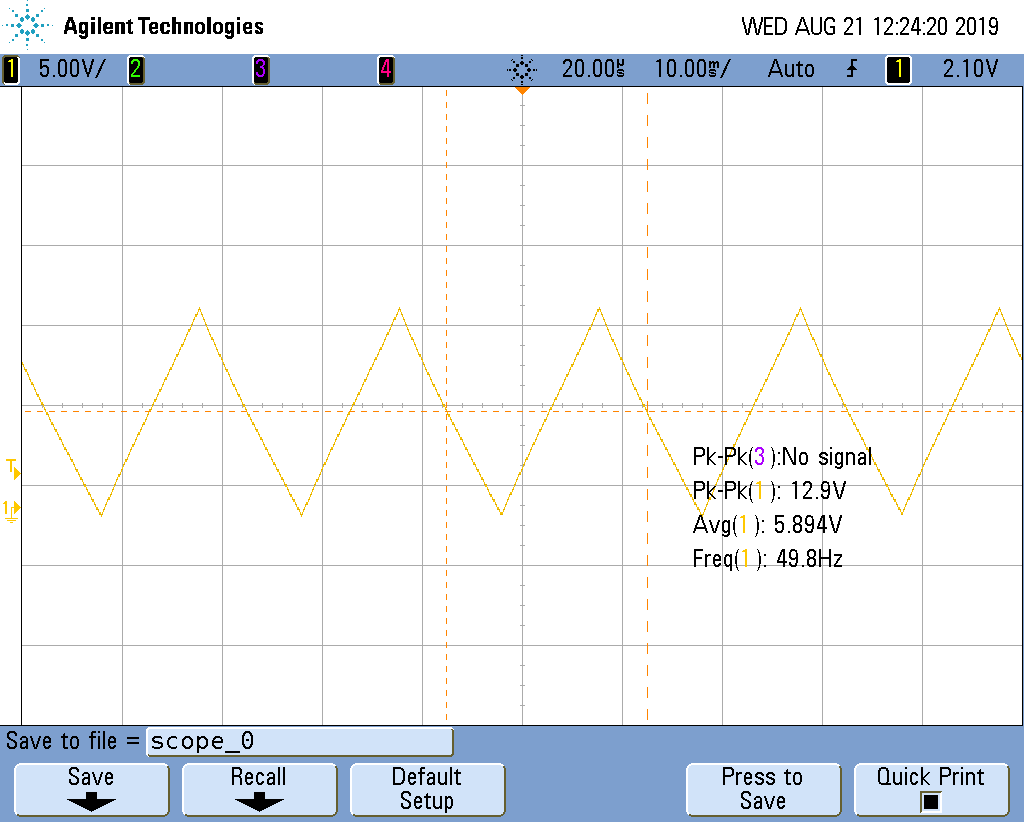
\includegraphics[width=0.5\textwidth]{Ej3/imagenes/opmpOscilando.png}
	\caption{Circuito Oscilando.}
	\label{fig:oscilando}
\end{figure}
Luego se volvió a medir en otro horario para el cual el ruido de linea no era tan intenso y  se pudo realizar una medición certera. Obteniendo para los valores de salida para la medición de $I_b^+$ y $I_b^-$. El aumento en el ruido de linea puede deberse a el instrumental que estaba siendo utilizado en el momento en el laboratorio.
\begin{figure}[H]
\centering
\begin{minipage}{.5\textwidth}
  \centering
  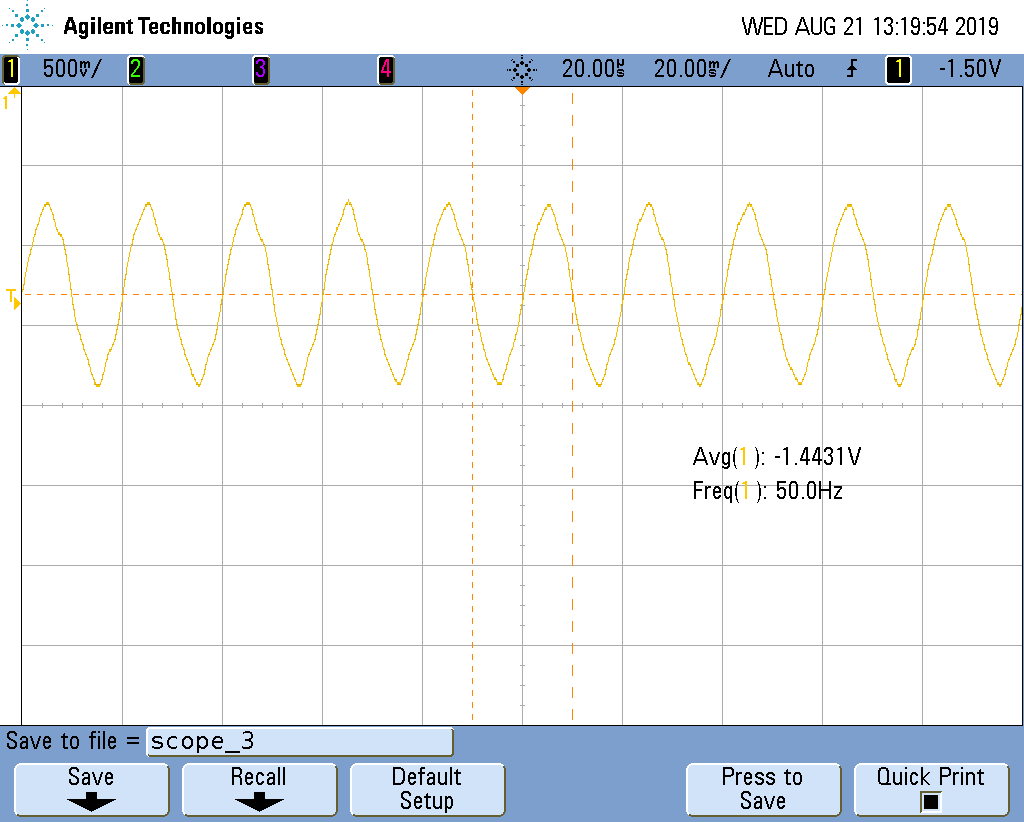
\includegraphics[width=.99\linewidth]{Ej3/imagenes/IB+.png}
  \captionof{figure}{Medición de Vout para Ib+}
  \label{fig:ib+}
\end{minipage}%
\begin{minipage}{.5\textwidth}
  \centering
  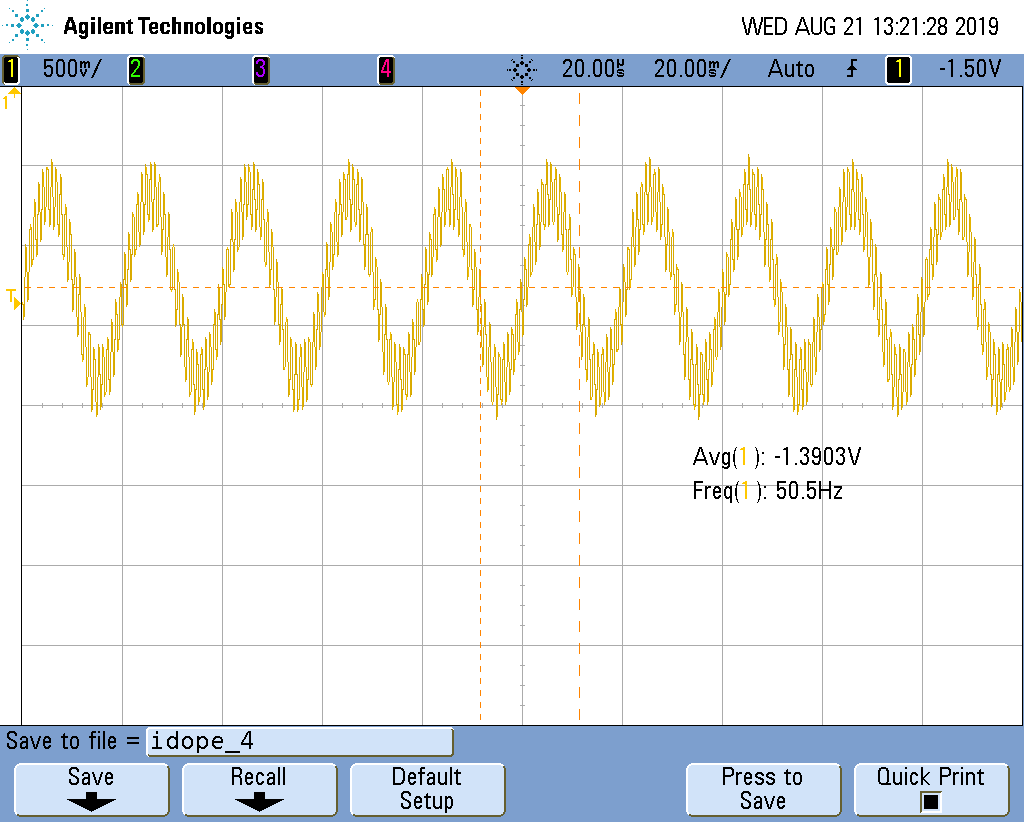
\includegraphics[width=.99\linewidth]{Ej3/imagenes/IB-.png}
  \captionof{figure}{Medición de Vout para Ib-}
  \label{fig:ib-}
\end{minipage}
\end{figure}


\subsubsection{Analisis de resultados.}
A partir de los valores obtenidos en la   \ref{tab:vout} se pueden calcular las corrientes de offset y bias, al igual que la tension de offset.
\begin{table}[H]
\begin{center}
\begin{tabular}{|c|c|c|c|l|}
\hline
\textbf{$V_{offset}$} & \textbf{$I_b^+$} & \textbf{$I_b^-$} & \textbf{$I_{bias}$} & \textbf{$I_{offset}$} \\ \hline
-1.44mV & -159pA & -100pA & -130pA & 58.6pA \\ \hline
\end{tabular}
\end{center}
\end{table}
Luego comparándola con la siguiente tabla de valores proporcionada por el fabricante:
\begin{table}[H]
\begin{center}
\begin{tabular}{|c|l|l|c|l|l|}
\hline
\multicolumn{6}{|c|}{\textbf{Datos de fabricante}}                                                                                                                                                       \\ \hline
\multicolumn{3}{|c|}{\textbf{Máximo}}                                                                & \multicolumn{3}{c|}{\textbf{Típico}}                                                              \\ \hline
\multicolumn{1}{|l|}{\textbf{$V_{offset}$}} & \textbf{$I_{bias}$}        & \textbf{$I_{offset}$}     & \multicolumn{1}{l|}{\textbf{$V_{offset}$}} & \textbf{$I_{bias}$}       & \textbf{$I_{offset}$}    \\ \hline
10mV                                        & \multicolumn{1}{c|}{200pA} & \multicolumn{1}{c|}{50pA} & 3mV                                        & \multicolumn{1}{c|}{20pA} & \multicolumn{1}{c|}{3pA} \\ \hline
\end{tabular}
\end{center}
\end{table}
Se puede observar que la mayoría de los valores se encuentran dentro de las tolerancias admitidas por el fabricante, el desvío en la corriente de offset es atribuido a los componentes que su valor no es preciso, que no se tuvo en cuenta a la punta del osciloscopio en el modelo.
\subsection{Compensación de tension de offset y corrientes de bias.}
\subsubsection{Compensación Bias}
Para la compensación de corriente de bias lo que se desea es hacer que la diferencia entre $I_b^+$ y $I_b^-$ sea $\approx$ 0
Un ejemplo de esto es tomar un Op Amp en configuración inversora  de las siguientes características:
\begin{figure}[H]	
	\centering
	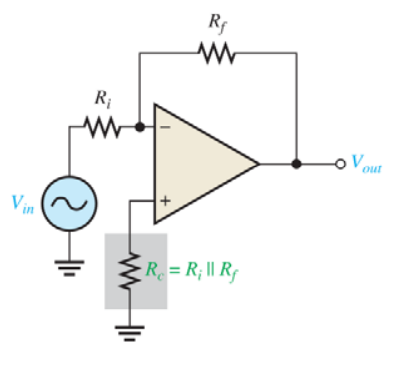
\includegraphics[width=0.5\textwidth]{Ej3/imagenes/CompensacionBias.PNG}
	\caption{Circuito inversor para la compensación de BIAS.}
	\label{fig:CompensacionBias}
\end{figure}
Asumiendo ya compensada la tensión de offset se procede a la deducción de el valor de Rc para minimizar las corrientes de bias.
\begin{center}$V_{out}=A_0 \cdot (V^+ - V^-)$\\\end{center}
\begin{center}$V^+=-I_b^+ \cdot R_c$\\\end{center}
\begin{center}$\frac{V_{in}-V^-}{R_i}=\frac{V^- - V_{out}}{R_f} -I_b^-$\\\end{center}
Despejando para $V_{out}$ queda:
\begin{center}$V_{out}=V_{in}\cdot -\frac{R_f}{R_i}+I_b^+ R_f-I_b^- R_c \cdot \frac{R_i+R_f}{R_i R_f}\cdot R_f $\\\end{center}
Teniendo un valor de $R_c$= $R_i//R_f$ se deberían anular o atenuar significativamente las corrientes de bias.
\subsubsection{Compensación Tension de Offset}
Para la compensación de la tensión de offset hay varias alternativas. En el caso de los Opamps que fueron usados en este informe cuentan con unos pines para configurar la tensión de offset(1 y 5), la forma que se va a desarrollar es un circuito externo que funcione en configuración inversora.
El circuito a implementar es el siguiente:
\begin{figure}[H]	
	\centering
	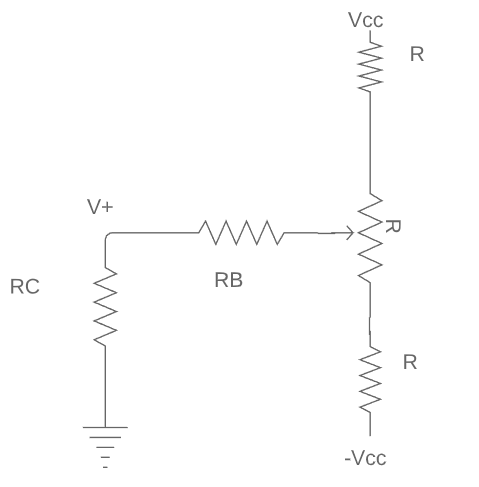
\includegraphics[width=0.5\textwidth]{Ej3/imagenes/CompensacionOff.PNG}
	\caption{Circuito para la compensación de tensión de offset.}
	\label{fig:CompensacionOff}
\end{figure}
El potenciómetro sera utilizado para variar la tension que se le agrega a $V^+$ a través del divisor resistivo conformado por $R_C$ y $R_B$ donde Rc podría ser una resistencia para compensar el BIAS. RB debe ser un valor por lo menos 10 veces superior a RC dado que la tensión que se quiere corregir es pequeña. el propósito de las 2 resistencias 'R' es aumentar la sensibilidad para elegir la tensión. El valor del potenciómetro debería ser un orden de magnitud menor que $R_B $

